\documentclass[10pt]{scrartcl}

\usepackage{graphicx}

\title{Scientific Experimentation and Evaluation\\
	   \small{Assignment: 1}}
\author{Chaitanya Hebbal\\
		Jos\'e Carlos Mayoral Ba\~nos}

\begin{document}
	\maketitle
\section*{What plan to do?}

Our \textbf{task} is defined as: \textit{Constructing a LEGO NxT differential drive robot and manually measure the observable pose variation for three different velocity motions}. The goal is to observed the variation on the manual measured poses and look at the error distributions that is leaded by the those.

In order to achieved the goal, there are some constraints that must be taken into account:

\begin{itemize}
	\item The Device Under Test is a LEGO NxT robot.
	\item DifferentialPilot library for motion behaviour.
	\item Manual measurement comes out with additional error provided by the person who makes them.
	\item The time of every movement must be constant.
	\item There is not a true value to compare with, this must be obtained from the repetitions of the experiment.
\end{itemize}

In order to accomplish the constraints, our plan to follow consists on:

\begin{enumerate}
	\item Define the measurement method (see below).
	\item Achieve a good code which takes into consideration the provided restrictions.
	\item Seven different curves movements are going to be measured: Straight line and 6 arcs (3 left and 3 right).
	\item Define the curves that must be done according to functions parameters.
	\item Twenty repetitions of every curve must be done.
	\item Store the information of the final poses.
	\item Compute the information to get the error gaussian distribution.
\end{enumerate}

\section*{Measurement System}

The measurement value (final pose) is acquired by a LEGO NxT robot which uses the libraries provided by leJOS framework for motion and a large cardboard sheet, light sensor and geometric representation to acquire data. 

\section*{Measuring Method}

To accomplish the task we have defined the experiment as explained in the picture.\\

\begin{figure}[h!]
\centering
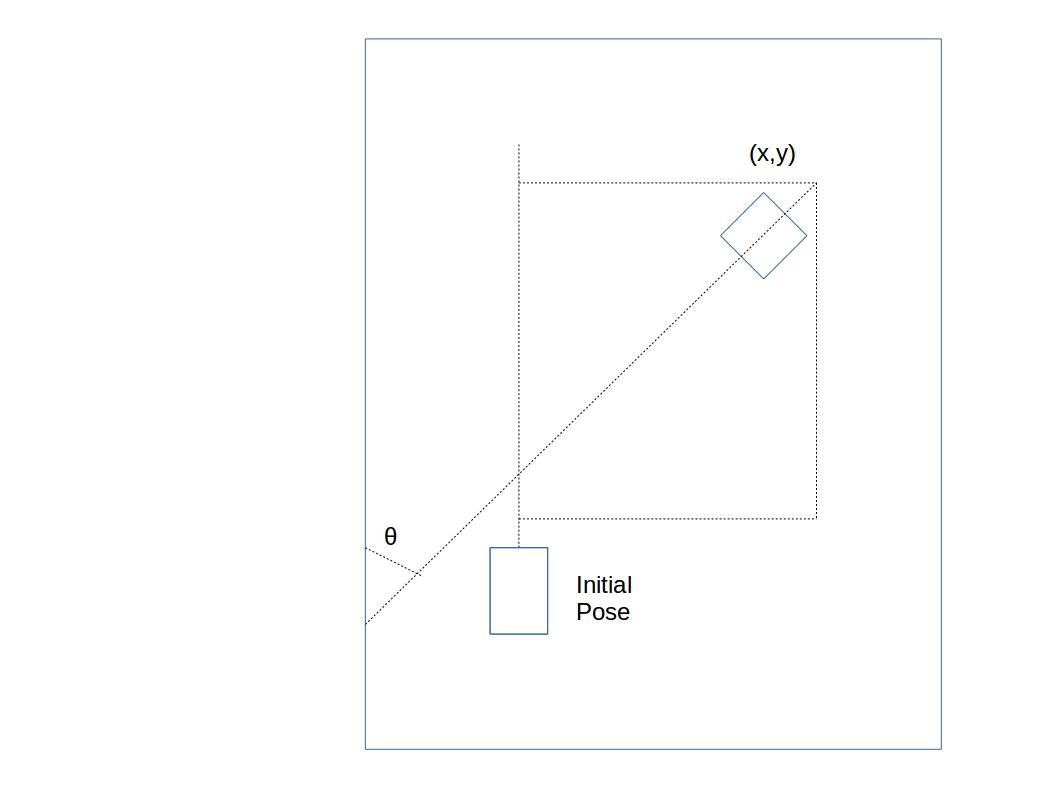
\includegraphics[trim=200 0 0 0, scale=0.35]{image}
\caption{Experiment Description}
\label{fig}
\end{figure}

The method description of image \ref{fig} is:
\begin{itemize}
	\item One LEGO structure will set the robot at initial position so the initial position will be constant.
	\item A cardboard is used to mark the points of all the experiment.
	\item Two light sensors are used to mark the points in order to get the pose of the robot.
	\item Project the line that is created between the two measured points.
	\item The angle will be measured with the projected line.
\end{itemize}

The Measurement facilities include:

\begin{itemize}
	\item One cardboard.
	\item Two light sensors.
	\item A pen.
	\item A protractor.
\end{itemize}

\section*{What difficulties are expected?}

In order to accomplish the current task, we found the following constraints:

\begin{itemize}
	\item The manual measurement will add errors to the measurement result.
\end{itemize}
	
\end{document}